\documentclass[12pt]{article}		% Précise le type de document, et la taille de la police de caractère
\renewcommand{\baselinestretch}{1,5}
\usepackage{rotating}
\usepackage{natbib} % Pour pouvoir utiliser une bibliographie externe
\usepackage[french]{babel}	% Pour préciser la langue du document
\usepackage[utf8]{inputenc}	% Précise comment le texte est saisi : cela permet de tapper directement les accents
\usepackage[T1]{fontenc}	% Précise la façon dont le document actuel est encodé
\usepackage{setspace}
\usepackage[margin=2.5cm]{geometry} % Précise les marges du document
\title{Titre}% N'affecte pas la page titre, mais défini le nom de votre projet
\author{Prénom Nom} % N'affecte pas la page titre, mais défini le nom de l'auteur(e) du projet

%Bibliographie
%----------------------------------------------------------------
\bibliographystyle{apalike-fr.bst} % Pour changer le style de bibliographie
\addto{\captionsfrench}{\renewcommand{\refname}{Bibliographie}} % Comme le langage défini est le français, "Références" aurait été le titre par défaut pour la bibliographie
\usepackage[numbib]{tocbibind} % Ajoute un numéro à bibliographie à la table des manière avec numéro 
% \usepackage[nottoc]{tocbibind}  Ajoute la bibliographie dans la table des matières sans numéro

%----------------------------------------------------------------

%Sections
%----------------------------------------------------------------
%\usepackage{newclude} % Pour pouvoir utiliser l'étoile après \inculde pour éviter les sauts de page. Ce package a des problême de compatibilité avec la package natbib
%\renewcommand\thesection{} % Pour éviter la numérotation des sections
%----------------------------------------------------------------

%Informations destinées à la page de présentation
%----------------------------------------------------------------
\newcommand{\titre}{Devis de recherche}
\newcommand{\auteurs}{Nom_de_Famille}
\newcommand{\matricules}{Matricule_élève}
\newcommand{\destinataire}{Prénom_NomProfesseur}
\newcommand{\cours}{POL-1234}
%----------------------------------------------------------------

%Autres packages et commandes utiles
%----------------------------------------------------------------
\usepackage{amsmath,amsthm,amssymb,amsfonts}	% Pour pouvoir inclure certains symboles et environnements mathématiques
\usepackage{enumerate} % Pour mieux gérer la commande enumerate dans les sections
\usepackage{graphicx}	% Pour inclure des images
\usepackage{color}	% Pour inclure du texte en couleur
\usepackage{units}	% Pour pouvoir tapper les unités correctement
\usepackage{pgf,tikz}	% Utilisation du module tikz, qui permet de tracer des belles images
\usetikzlibrary{arrows} % Quand on exporte une image GeoGebra, on a besoin de préciser cela
\usepackage{hyperref}	% Pour include des liens dans le document
\newcommand{\N}{\mathbb{N}}	% Commande personnelle, plus rapide pour tapper les ensembles
\newcommand{\Z}{\mathbb{Z}}	% Commande personnelle, plus rapide pour tapper les ensembles
\newcommand{\R}{\mathbb{R}}	% Commande personnelle, plus rapide pour tapper les ensembles
\usepackage{cprotect}	% Pour pouvoir personaliser la légende des figures
\usepackage{pdfpages} 
%----------------------------------------------------------------


\begin{document}
\thispagestyle{empty}	% Pour éviter d'avoir un en-tête et un pied de page sur la page couverture

\includegraphics[width=9cm]{img/calais.png}	% Pour inclure le logo (on précise la largeur de l'image)
\vspace{2cm}	% Espacement vertical
\begin{center}	% On centre le texte
{\huge \bf\ Projet Erub}  \\
{\Large \bf\ \\Licence Professionnelle DIM Développement Internet et Mobile}  \\% \huge fait que le texte est gros, \bf fait que le texte est gras
\vspace{3cm}
\large Travail présenté à Antoine Gamelin \\
\vspace{3cm}
réalisé par \\ \ CARUYER Claire 
\vfill	% On va jusqu'au bas de la page avant de mettre le texte ci-dessous
\today
\pagebreak
\end{center} % Inclut le code contenu dans un fichier comme s'il était entré ici

%\section{Résumé}
J'ai appris a développer un bot discord avec node js. J'ai choisit d'apprendre à développer un bot discord car je passe énormément de temps dessus.
%\newpage

\tableofcontents 
% Le package newclude mis en commentaire permet d'introduire une * pour éviter le saut de page entre les section
\pagebreak
%\maketitle
%% Devis de recherche


\section{Introduction}

    Dans le cadre du Module Complément Informatique au cours de ma formation en Licence
Professionnelle DIM (Développement Internet et Mobile) à l'IUT de Calais, j'ai réaliser un bot discord en passant par l'API discord.

    Pour ce projet nous pouvions choisir entre plusieurs API, mon choix c'est porté sur
Discord car je passe beaucoup de temps dessus et que c'est un bon sujet pour le développement avec node js.
\newpage
\section{Discord - Erub}

Discord est un logiciel propriétaire gratuit de VoIP et de messagerie instantanée. Il fonctionne sur les systèmes d’exploitation Windows, macOS, Linux, Android, iOS ainsi que sur les navigateurs web.

Pour développement de mon bot discord, je suis passée par l'API discord.\\

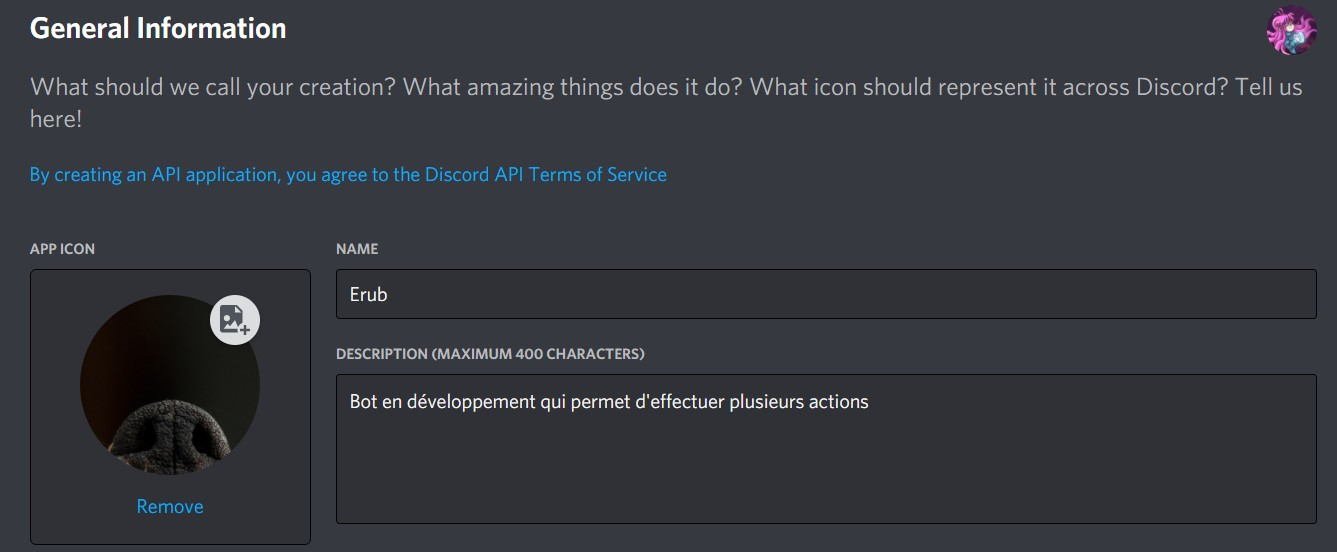
\includegraphics[width=16cm]{img/api.jpg}	

L'api permet d'avoir un token permettant de relier le bot que l'on développe à l'api pour permet au bot de rejoindre des serveurs. Le token est important, il ne faut pas rendre public.

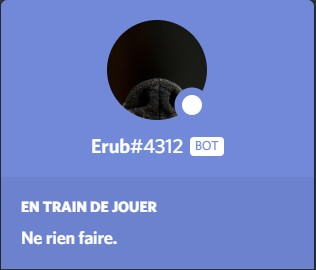
\includegraphics[width=5cm]{img/Erub.jpg}	

Structure de Erub: 
- commandes : Ce dossier contient toutes les focntionnalitées du bot triées dans d'autres dossiers.

- config.js : Contient les paramètres a initiliser si vous voulez tester le bot sur votre serveur.

- node\_modules : contient tous les packages node js dont nous avons besoin

- package.json : contient les dépendences et leur version ainsi que des scripts

- main.js : Point d'entrée de l'application.

J'ai appris à mettre des statuts personnalisées sur mon bot. 
Cela peut permettre à des utilisateurs ne connaissant pas le bot d'avoir des informations, par exemple j'affiche la commade "?help"

Erub peut également afficher un message de bienvenue aux utilisateurs pour cela il suffit de mettre l'id du channel dans le config.js

Il peut également afficher les sondages dans un channel dédier ou alors la ou vous taper la commande si vous initialisez à num le paramètre "CHANNEL\_POLL" dans le fichier config.json.

\newpage
\section{Fonctionnalités}
Les différentes fonctionnalités de {\bf Erub} sont : \\
{\bf Administratif} : commandes réservés au propriétaire/créateur du serveur
    \begin{itemize}
        \item{\bf ?purge nombre}  Permet de supprimer entre 1 et 100 messages de moins de 14 jours d'un channel
        
        \item{\bf ?eval arguments}  Cette commande permet à l'utilisateur d'effectuer n'importe quel calcul.
        ex: {\bf?eval (5*6)/2+5*((4/2)+5) = 50}
        
    \end{itemize}
    
    
\includegraphics[width=6cm]{img/purge.jpg}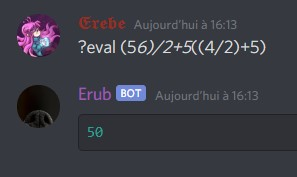
\includegraphics[width=7cm]{img/eval.jpg}
    
{\bf Jeux}: 
    \begin{itemize}
        \item {\bf ?chifumi} Permet de jouer aléatoirement donc le bot au chifoumi
        \item {\bf ?pierre} Permet de jouer pierre contre le Bot
        \item {\bf ?feuille} Permet de jouer feuille contre le Bot
        \item {\bf ?ciseaux}  Permet de jouer ciseaux contre le Bot
        \item {\bf ?pile} ou {\bf ?face} permet de lancer une pièce
        
    \end{itemize}
    
     
\includegraphics[width=6cm]{img/face2.jpg}
\includegraphics[width=7cm]{img/pile.jpg}
    \newpage
{\bf Sondages}: 
    \begin{itemize}
        \item {\bf ?poll votre question} Permet de générer un sondage avec pour réponses  oui ou non

        \item {\bf ?poll2 votre question/votre réponse 1/votre réponse 2/votre réponse 3} Permet de générer un sondage avec des arguments, vous pouvez définir jusqu'à 10 réponses qui seront numérotés de 1 à 10.
        
    \end{itemize}
    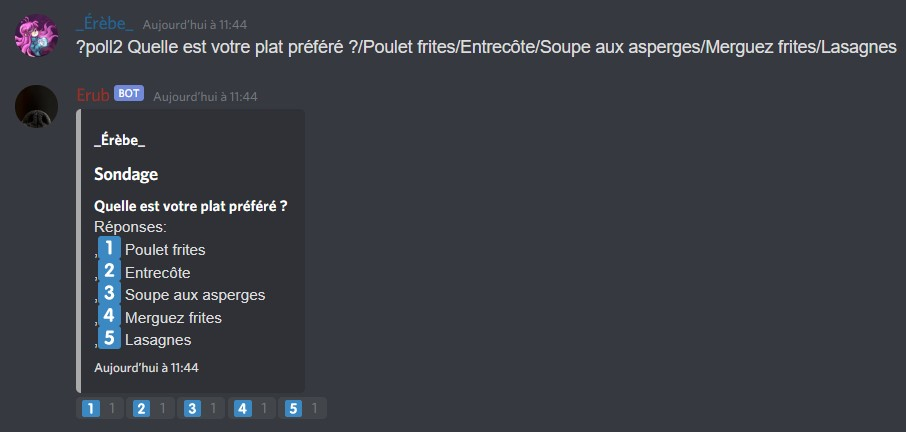
\includegraphics[width=10cm]{img/poll2.jpg} 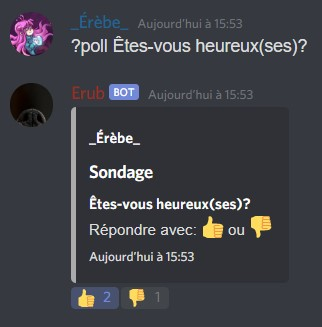
\includegraphics[width=5cm]{img/poll.jpg}
    
{\bf Informatif}: 
    \begin{itemize}
        \item{\bf ?help}  Cette commande permet à un utilisateur de demander les commandes disponibles par le bot
        
        \item {\bf ?botinfo} Permet d'afficher les informations du bot
        
        \item {\bf ?userinfo} Permet d'afficher nos informations Discord 
        
        \item {\bf ?userinfo @autre\_user} Permet d'avoir les informations d'un autre utilisateur du serveur.
        
        \item {\bf ?serverinfo} Permet d'afficher les informations du serveur

    \end{itemize}
    
    Affichage des informations utilisateurs: 
    
    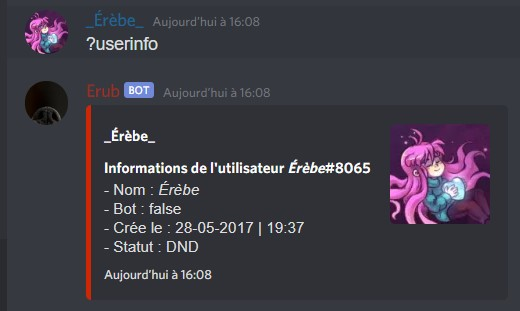
\includegraphics[width=8cm]{img/userinfo_dnd.jpg}
\includegraphics[width=9cm]{img/userinfo_idle.jpg}
    
    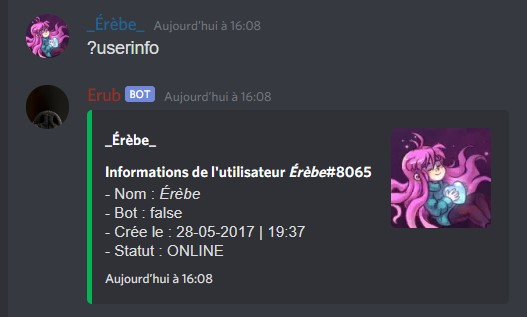
\includegraphics[width=8cm]{img/userinfo_online.jpg}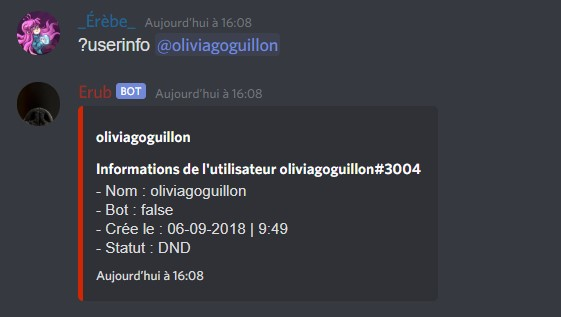
\includegraphics[width=9cm]{img/userinfo_otheruser.jpg}
    
    Commande help: 
    
    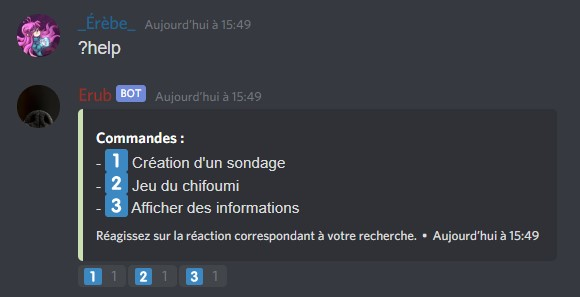
\includegraphics[width=10cm]{img/help.jpg}
    
    Informations du serveur:
    
    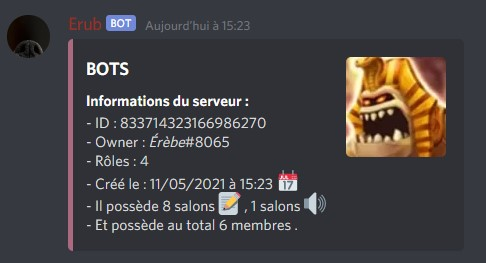
\includegraphics[width=10cm]{img/serverinfo.jpg}
    
    Informations bots, pages allant de 1 à 5: 
    
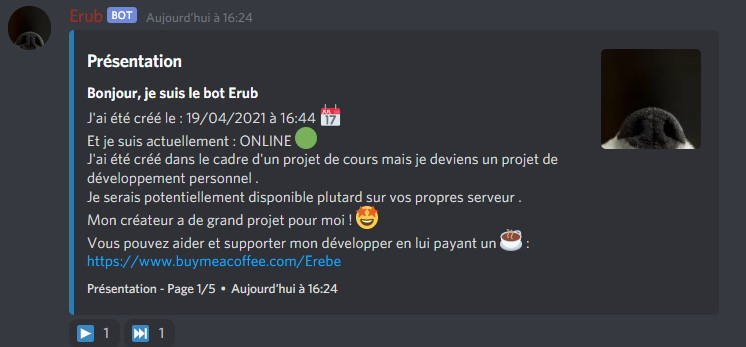
\includegraphics[width=9cm]{img/botinfo_page_1.jpg}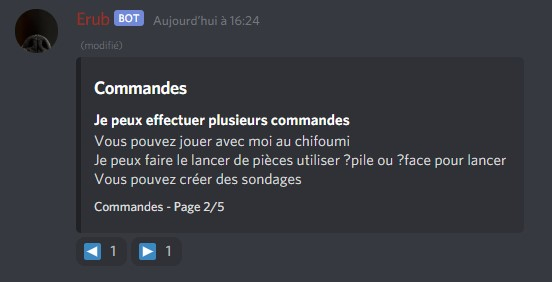
\includegraphics[width=8cm]{img/botinfo_page_2.jpg}
    
    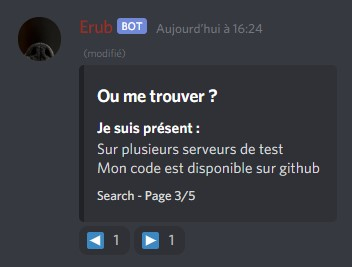
\includegraphics[width=7cm]{img/botinfo_page_3.jpg}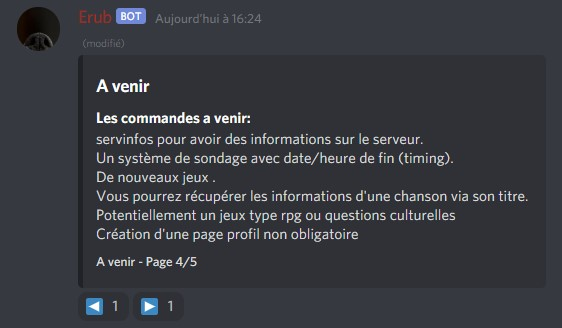
\includegraphics[width=10cm]{img/botinfo_page_4.jpg}
    
    
\includegraphics[width=12cm]{img/botinfo_page_5.jpg}
\newpage
\section{Difficultées}
    La principale difficulté que j'ai rencontré est survenu au début du projet car je voulais tout de
suite intégrer une base de données et mettre en place un sondage très élaborées avec une fin de soudage sauf que cela était plus compliqué que prévu.
    Je préfois donc d'utiliser une bdd plus tard.

    J'ai rencontrée des difficultés pour récupérer les informations des utilisateurs, en occurrence avoir leur statut. En effet tous les utilisateurs s'affichaient avec le statut "offline" alors que parfoisl'utilisateur était : 
    
        - connecté en dispo
        
        - connecté en occupé 
        
        - ou absent 
        
    Il s'agissait en fait d'un paramètre a activé sur l'api discord pour permet au BOT d'avoir accès aux informations de l'utilisateur. 
    
    J'ai finalement réussit à créer un sondage à réponses multiples mais il n'y a pas de temps pour répondre ni de date de fin et les sondages ne sont stockés null part. Le nombre de réponse possible est limité à 10 car il n'y a pas de réaction surpérieur à "10" en chiffre, il faudra sinon utiliser d'autres réactions.
    
    
    J'ai essayé de connecté mon bot à une autre api qui permettait de récupérer des informations sur des chansons tels que son auteur et ses paroles mais la connection echouait à chaque fois, l'api refusait la connection alors que les token et clés étaient passées en paramètres. 
    Je dois donc ré essayer ou trouver d'ou pourquoi l'api rejette la connexion. 
    
\section{Conclusion}
    A la fin de se module, nous nous retrouvons avec un bot comprennant plusieurs commandes. Il reste encore des fonctionnalitées à améliorer et à venir mais le bot est fonctionnel.
\pagebreak
\end{document}